\author{Florian Müller and Paul Hoffmann}
\chapter{Exam-Container}

\begin{figure}[H]
    \centering
    \subfloat{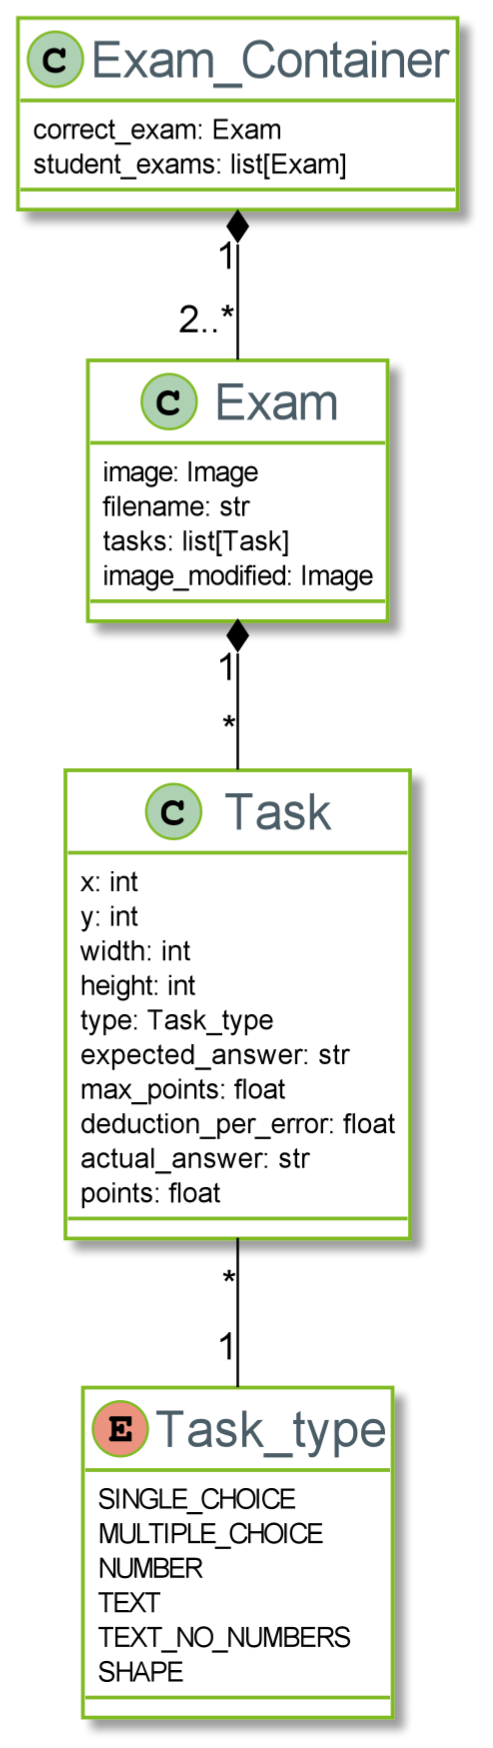
\includegraphics[width=0.35\linewidth]{src/chapters/developer/media/exam_container.png}}
    \caption{Object diagram of the ExamContainer}
\end{figure}

The ExamContainer is the main class for the communication.
This class contains the sample solution and a list of exams for the correction.

An exam is the class for storing an exam.
It contains the image of an exam, the filename, a list of tasks and the modified image.

Inside the task class are the values for the region of interest.
Beside that also the expected answer from the sample solution.
Finally the points for the single task and the deduction per error are saved.
When the exam was corrected the resulting points are also saved here.

The task-type describes the available tasks for the backend processing.
Beside the task "SHAPE" every task was implemented inside the backend.
